%!TEX root = ../thesis.tex
\chapter{Розробка та порівняльний аналіз моделей машинного навчання навчання}
\label{chap:practice}

\section{Підготовка датасету}

Для формування датасету використано два основних джерела даних:
супутникове зображення та відповідну маску з розміченими кратерами.
Важливо зазначити, що в межах даної роботи використані дані,
сформовані науковим колективом кафедри ММАД.
Початковий датасет був фрагементований
на патчі розміром 128x128 пікселів. Такий розмір був обраний довільно,
моделі, представлені у даній роботи, підтримують зображення будь якого
розміру, з умовою, що розширення ділиться на 32 націло.
Відбір
патчів для подальшої обробки відбувався на підставі критерію, згідно
з яким у вибраних патчах область, що відповідала масці, становила не
менше 10\% загальної площі. Цей підхід сприяє виокремленню
суттєвих особливостей і забезпечує відсутність у датасеті
зображень, які не мають достатнього для навчання матеріалу. У результаті цього етапу формування
було отримано 1000 патчів. Наступним кроком було розділення
отриманого датасету на тренувальні, валідаційні та тестові підмножини
відповідно у відношенні 80\%:10\%:10\%. Ця стратегія розподілу дозволяє
забезпечити ефективне навчання моделі та об'єктивну оцінку її продуктивності
на випробувальних даних. Програмна реалізація даного модулю представлена у додатку А.1.

\section{Реалізація моделей}

У рамках дослідження використано три широко відомі моделі для
сегментації зображень: FPN, U-Net та DeepLabv3,
усі з базовою згортковою архітектурою ResNet-34.
ResNet-34 -- це глибока згорткова нейронна мережа, навчена на наборі
даних CIFAR-10~\cite{he2015}. Це частина сімейства ResNet,
яке вирішило проблему зникнення градієнтів у глибоких
нейронних мережах, що дозволяє ефективно навчати набагато
глибші мережі. Основна інновація ResNet-34 полягає
у використанні залишкового навчання. Замість того, щоб
вивчати пряме відображення від входу до виходу, залишкові
мережі вивчають різницю (або залишок) між входом і виходом.
Цей підхід реалізується за допомогою коротких з'єднань,
які оминають один або декілька шарів, що дозволяє мережі
вивчати залишкові функції з посиланням на входи шарів.

Архітектура ResNet-34 складається з 34 згорткових шарів,
організованих у серії залишкових блоків. Кожен блок містить
два згорткових шари, за якими слідує коротке з'єднання,
що додає вхід блоку до його виходу. Мережа починається
з початкового згорткового шару, за яким слідує шар
максимального об'єднання, а потім проходить через
чотири етапи залишкових блоків. Ці етапи містять 3, 4, 6
і 3 блоки відповідно, причому на кожному етапі кількість
фільтрів збільшується і подвоюється на кожному переході.
Мережа завершується глобальним середнім об'єднуючим шаром
і повністю з'єднаним шаром для цілей класифікації.

ResNet-34 показала чудову продуктивність у різних задачах розпізнавання
зображень, значно зменшивши помилки навчання завдяки вирішенню проблеми
зникаючого градієнта, яка є поширеною в глибоких мережах.

Для реалізації обраних моделей для завдання сегментації
зображень, а також використання функцій втрат Dice Loss і Focal Loss,
було використано пакет Segmentation Models
PyTorch~\cite{iakubovskii2019}, який
надає готові реалізації різноманітних архітектур
нейронних мереж для сегментації зображень на базі
бібліотеки PyTorch. Цей пакет дозволяє швидко та зручно
використовувати високоякісні моделі, а також зручно
налаштовувати параметри навчання та валідації.
Використання готових реалізацій у пакеті спрощує
процес розробки та дозволяє зосередитися на розв'язанні
основної задачі без необхідності вирішувати деталі
реалізації моделей.

Додатково, для забезпечення ефективного та
структурованого процесу навчання моделей та відладки
коду, використовувалася бібліотека PyTorch Lightning~\cite{falcon2019}.
PyTorch Lightning надає високорівневий інтерфейс для
навчання нейронних мереж на базі PyTorch, що дозволяє
зосередитися на архітектурі та параметрах моделі,
відділивши їх від деталей навчання. Завдяки цьому,
можна зручно використовувати різноманітні техніки
навчання, такі як автоматичне зберігання моделі,
відстеження метрик, розподіл тренування на різні
пристрої та багато іншого. Використання PyTorch
Lightning сприяло підвищенню продуктивності розробки
та навчання моделей для задачі сегментації зображень.
Програмна реалізація основного модулю програми наведену у додатку А.2.

Для об'єктивного порівняння точності моделей,
використаних у дослідженні, було застосовано метрику
Intersection over Union (IoU) на валідаційному датасеті.
Ця метрика вимірює ступінь перекриття між прогнозованою
та реальною сегментаційними масками і дозволяє отримати
об'єктивну оцінку якості сегментації. Формула IoU наступна:
\begin{equation*}
      \text{IoU} = \frac{|A \cap B|}{|A \cup B|}.
\end{equation*}

Також моделі були оцінени на тестовому датасеті, звідки отримано
значення метрик recall (повнота), precision (точність) і F1.

Повнота, також відома як чутливість або частота
істинних позитивних результатів, вимірює частку фактичних
позитивних результатів, які правильно ідентифіковані моделлю.
Формула повноти виглядає так:
\begin{equation*}
      \text{Recall} = \frac{TP}{TP + FN},
\end{equation*}
де $TP$ (True Positives) -- кількість
правильно передбачених позитивних пікселів,
а $FN$ (False Negatives) -- кількість фактичних
позитивних результатів, які були помилково
класифіковані як негативні.

Точність, також відома як позитивна прогностична цінність,
вимірює частку позитивних ідентифікацій, які
насправді є правильними.
Формула для точності має вигляд:

\begin{equation*}
      \text{Precision} = \frac{TP}{TP + FP},
\end{equation*}
де $FP$ (False Positives) -- кількість негативних пікселів,
які були помилково класифіковані як позитивні.

Оцінка F1 -- це середнє гармонійне значення точності та
повноти, що забезпечує єдину метрику,
яка збалансовує обидва показники. Вона
особливо корисний, коли класи незбалансовані,
оскільки враховує як хибнопозитивні, так і
хибнонегативні спрацьовування. Формула для
оцінки F1 має вигляд:

\begin{equation*}
      \text{F1} = 2 \times \frac{\text{Precision} \times \text{Recall}}{\text{Precision} + \text{Recall}}.
\end{equation*}
Ця метрика приймає значення від 0 до 1, де
вищий показник вказує на кращий баланс між
точністю та повнотою.

\section{Порівняльний аналіз моделей машинного навчання}

Спираючись на графік, зображений на рис.~\ref{iou_comp},
можна сказати, що моделі, які навчалися з Dice Loss,
навчаються більш стабільно, ніж ті, у яких функцією
втрат виступає Focal Loss.
Причинами цього можуть бути фактори, наведені нижче.

\begin{itemize}

      \item Чутливість моделі до складних прикладів:
            Focal Loss надає більшої ваги складним прикладам,
            які модель намагається правильно класифікувати.
            Таке підвищене фокусування може призвести до більш
            значних коливань у прогнозах моделі, особливо на
            ранніх стадіях навчання, коли параметри моделі все
            ще оптимізуються. Як наслідок, метрика IoU, яка є
            чутливою до якості прогнозів, може демонструвати
            більшу варіабельність і виглядати хвилясто.
      \item Швидкість навчання та динаміка оптимізації:
            вибір швидкості навчання та інших гіперпараметрів
            оптимізації може впливати на стабільність процесу
            навчання. Висока швидкість навчання може спричинити
            сильніші коливання параметрів моделі, що призведе до
            нестабільних показників ефективності. Навіть при добре
            підібраній швидкості навчання, притаманна динаміка
            фокусування на складних прикладах
            може внести нестабільність у процес навчання, що
            призведе до хвилястої кривої IoU.
      \item Ефекти регуляризації: методи регуляризації,
            такі як пулінг або доповнення даних, які
            часто використовуються для запобігання надмірному
            пристосуванню, можуть внести додаткову варіативність
            у навчальний процес. У поєднанні з Focal Loss,
            яка вже змінює оновлення градієнта, щоб зосередитися
            на важких прикладах, ця мінливість може відображатися
            на метриці IoU, роблячи її менш стабільною.

\end{itemize}

\begin{figure}[ht]
      \centering
      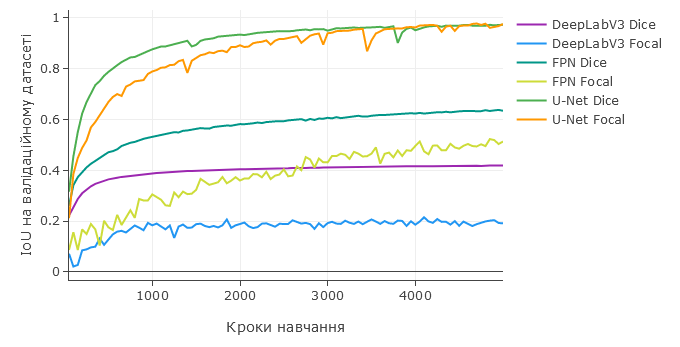
\includegraphics[scale=0.8]{Images/iou_comp.png}
      \caption{Порівняння значення IoU під час навчання}
      \label{iou_comp}
\end{figure}

За даними табл.~\ref{int_comp}, можна зробити наступні висновки.
Найбільш ефективною моделлю виявилась U-Net, при чому і з використанням
Dice Loss, і з використанням Focal Loss. Це свідчить про те, що
архітектура даної моделі найкраще підходить для вирішення поставленої
задачі, а модель добре підлаштувалась під навчальні дані. Високі показники
моделі на тестовому датасеті показають, що модель не перетренована.

Найгірше себе проявила модель DeepLabv3. Вона не тільки має найменші показники
повноти, точності та F1, але й має найбільший час навчання, майже вдвічі довше,
ніж інші представлені моделі.

Ще одним висновком є те, що моделі, які навчались з використанням Dice Loss,
показують кращі результати за ті, що навчались з використанням Focal Loss.

\begin{table}[ht]
      \setfontsize{12pt}
      \caption{Порівнняня метрик моделей глибокого навчання}
      \label{int_comp}
      \centering
      \begin{tabular}{|c|c|c|c|c|c|c|}
            \hline
            Функція втрат               & Назва моделі & Recall & Precision & F1   & IoU  & Час навчання (хв.) \\ \hline
            \multirow{3}{*}{Dice Loss}  & FPN          & 0.85   & 0.71      & 0.77 & 0.63 & 29.31              \\ \cline{2-7}
                                        & U-Net        & 0.98   & 0.99      & 0.99 & 0.97 & 34.37              \\ \cline{2-7}
                                        & DeepLabv3    & 0.78   & 0.47      & 0.59 & 0.42 & 53.86              \\ \hline
            \multirow{3}{*}{Focal Loss} & FPN          & 0.64   & 0.73      & 0.68 & 0.51 & 37.15              \\ \cline{2-7}
                                        & U-Net        & 0.98   & 0.99      & 0.99 & 0.97 & 40.1               \\ \cline{2-7}
                                        & DeepLabv3    & 0.22   & 0.58      & 0.32 & 0.19 & 54.48              \\ \hline
      \end{tabular}
\end{table}

На рис.~\ref{image_and_gt} зображений приклад знімку і істинної маски,
взятий з тестового датасету. На цьому прикладі були продемонстровані
прогнозовані маски моделей, навчених з використанням Dice Loss (рис.~\ref{pred_dice_comp})
і Focal Loss (рис.~\ref{pred_focal_comp}).

\begin{figure}[ht]
      \centering
      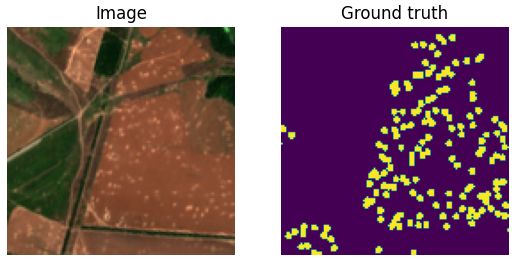
\includegraphics[scale=1]{Images/image_and_gt.png}
      \caption{Приклад знімку і істинної маски з тестового датасету}
      \label{image_and_gt}
\end{figure}

\begin{figure}[ht]
      \centering
      \begin{subfigure}[b]{0.33\textwidth}
            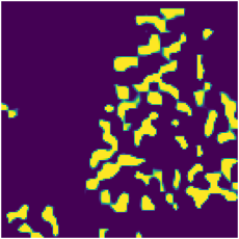
\includegraphics[scale=0.75]{Images/fpn_dice_pred.png}
            \caption{FPN}
      \end{subfigure}%
      \begin{subfigure}[b]{0.33\textwidth}
            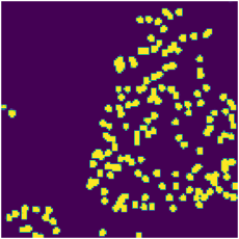
\includegraphics[scale=0.75]{Images/unet_dice_pred.png}
            \caption{U-Net}
      \end{subfigure}
      \begin{subfigure}[b]{0.33\textwidth}
            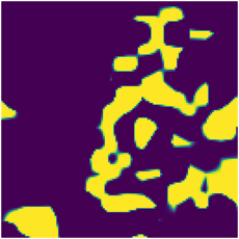
\includegraphics[scale=0.75]{Images/deeplab_dice_pred.png}
            \caption{DeepLabv3}
      \end{subfigure}

      \caption{Порівняння прогнозованих масок моделей з функцією втрат Dice Loss}
      \label{pred_dice_comp}
\end{figure}

\begin{figure}[ht]
      \centering
      \begin{subfigure}[b]{0.33\textwidth}
            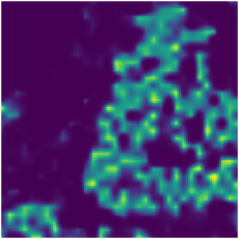
\includegraphics[scale=0.75]{Images/fpn_focal_pred.png}
            \caption{FPN}
      \end{subfigure}%
      \begin{subfigure}[b]{0.33\textwidth}
            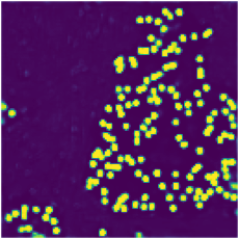
\includegraphics[scale=0.75]{Images/unet_focal_pred.png}
            \caption{U-Net}
      \end{subfigure}
      \begin{subfigure}[b]{0.33\textwidth}
            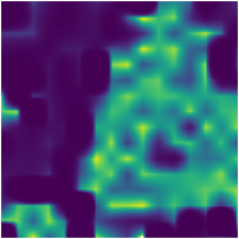
\includegraphics[scale=0.75]{Images/deeplab_focal_pred.png}
            \caption{DeepLabv3}
      \end{subfigure}

      \caption{Порівняння прогнозованих масок моделей з функцією втрат Focal Loss}
      \label{pred_focal_comp}
\end{figure}

Зважаючи на представлені приклади, наочно видно переваги Dice Loss
над Focal Loss. Хоча U-Net має приблизно ідентичні показники
ключових метрик, прогнозована маска у моделі, як навчалась з Dice Loss,
має чіткіші межі кратерів і не має відхілень, на відміну від моделі
з Focal Loss. Результати інших двох моделей, FPN та DeepLabv3,
суттєво відрізняються в залежності від функції втрат. Результати
з Dice Loss набагато чіткіші, хоча й мають проблеми з
розрізненнями індивідуальних кратерів. Причинами такої поведінки
є наступнє:

\begin{itemize}

      \item Dice Loss дуже чутлива до просторового перекриття між прогнозованими та
            фактичними сегментами. Ця чутливість спонукає модель створювати більш точні
            прогнози як за формою, так і за розташуванням, що має вирішальне значення для
            задач, де потрібна точна сегментація.
      \item У випадках, коли об'єкти сегментації є
            невеликими та розрідженими, Dice Loss може
            бути особливо ефективною. Вона гарантує,
            що модель приділяє належну увагу малим регіонам,
            уникаючи зміщення в бік більших регіонів, яке може
            виникнути з іншими функціями втрат, такими як Cross-Entropy Loss і Focal Loss.
      \item Dice Loss за своєю суттю врівноважує внесок суттєвих класів і фону. У задачах
            сегментації, особливо при роботі з медичними зображеннями або виявленні рідких
            об'єктів, об'єкт інтересу часто займає набагато меншу площу порівняно з фоном.
            Dice Loss відповідним чином масштабує важливість суттєвих класів, гарантуючи,
            що невеликим структурам надається більше значення в процесі навчання.

\end{itemize}

Хоча Focal Loss ефективна для обробки дисбалансу
класів і фокусування на складних прикладах, вона
не оптимізує безпосередньо перекриття між прогнозованими
і фактичними сегментами. Іноді це може призвести до менш
оптимальної продуктивності в задачах сегментації порівняно
з Dice Loss, яка спеціально розроблена для максимізації перекриття
по регіонах.

У контексті даної роботи, U-Net краще справляється з
сегментацією кратерів. U-Net була спеціально розроблена
для сегментації біомедичних зображень, де часто зустрічаються
невеликі об'єкти. Її архітектура, що характеризується симетричними
кодерно-декодерними шляхами з пропускними з'єднаннями,
чудово зберігає просторову інформацію та захоплює дрібні деталі.
Пропускні з'єднання допомагають зберегти характеристики
високої роздільної здатності від кодера і поєднати їх з
характеристиками декодера, що має вирішальне значення для
точної сегментації дрібних об'єктів.

В той же час, і DeepLabV3, і FPN передбачають багаторазове
зменшення вибірки для вилучення об'єктів, що може призвести
до втрати просторової роздільної здатності. Хоча ці
архітектури використовують методи відновлення просторової
інформації (наприклад, збільшення вибірки і використання
карт об'єктів з вищою роздільною здатністю), початкова
втрата деталей може вплинути на якість сегментації для
невеликих об'єктів. Архітектура U-Net, з її орієнтацією на
збереження інформації з високою роздільною здатністю завдяки
використанню пропускних з'єднань, краще підходить для
вирішення цієї проблеми.

\section*{Висновки до розділу 3}

Отже, у даному розділі було
описано процес розробки та проведено порівняльний аналіз
моделей машинного навчання для розв'язання задачі
сегментації кратерів на супутникових зображеннях.
Датасет, який початково
складався із одного знімку та відповідної розміченої маски, було
поділено на випадкові патчі розміру 128x128, і обрані ті з них,
де маска складала хоча б 10\% від загальної картинки.
Таким чином, було отримано достатньо даних для навчання, валідації та
тестування обраних моделей. Імплементація моделей та функції втрат відбувалась за допомогою
бібліотек Segmentation Models PyTorch і PyTorch Lightning, які
значно спростили побудову та навчання моделей.

Найбільш ефективною моделлю виявилась U-Net з використанням Dice Loss,
а найменш ефективною -- DeepLabv3 з використанням Focal Loss.
U-Net дає змогу точно визначити місцеположення кратерів, в той час
як інші дві моделі можуть надавати лише приблизні зони впливу,
а окремі кратери виділяються дуже рідко.
Також, варто зазначити, що моделі, які навчалися з Dice Loss
показують кращі і більш стабільні результати ніж ті,
що навчались з Focal Loss.